\renewcommand{\SS}{\mathbb{S}}
\newcommand{\Par}[2]{\mbox{$( #1, #2 )$}}
\usetikzlibrary{positioning, shapes, trees, graphs} % RNA trees
\newcommand{\scale}{0.6}

\newcommand{\tree}[1]{\ensuremath{#1}}

\chapter{Úvod do štúdia RNA štruktúry a grafov}

V~tejto časti práce zoznámime čitateľa s pojmami, ktoré s~RNA a~jej
štruktúrou súvisia.




\section{Čo je RNA}

RNA, ribonukleová kyselina, je jednovláknová molekula, pozostávajúca
zo sekvencie nukleotidov, jej základných stavebných častí.
Tie sa ďalej skladajú z~cukru (pentózy), dusíkatej bázy a~zvyšku
kyseliny fosforečnej. Poznáme štyry druhy báz,
adenín, cytozín, guanín a uracyl, označovať ich budeme A, C, G a U.
Okrem báz nás ďalšie zložky nebudú zaujímať a~tak ďalej v texte stotožníme
pojmy nukleotid a~báza.

Štruktúru RNA môžeme chápať podľa stupňa zjednodušenia
\begin{itemize}
  \item Primárna štruktúra - poradie nukleotidov v reťazci
  \item Sekundárna štruktúra - párovanie medzi bázami
  \item Terciárna štruktúra - priestorové usporiadanie molekuly
\end{itemize}

RNA ako jednovláknová molekula sa v snahe minimalizovať voľnú energiu páruje sama na seba.
V~tomto hrajú úlohu vodíkové väzby medzi nukleotidmi. Tie majú vzájomnú preferenciu,
čo znamená, že páry vznikajú najčastejšie medzi A-U a C-G, no ani iné
kombinácie nie sú vylúčené. 




\section{Sekundárna štruktúra}

Hlavným objektom nášho záujmu je sekundárna štruktúra RNA. V~nasledujúcej
časti si ju definujeme formálnejšie.

\begin{definice}
  \label{def:RNA_sekundarna_struktura}
  Primárna štruktúra RNA je určená poradím nukleotidov v~polynukleotidovom reťazci.
  \\
  Sekundárnou štruktúrou označíme množinu $\SS$ párov báz \Par{i}{j} takých,
  že pre dva páry \Par{i}{j} a \Par{k}{l} $\in \SS$ (bez straty všeobecnosti $i \leq k$)
  platí jedno z~nasledujúcich:
  \begin{itemize}
    \item $i = k \iff j = l$
    \item $i < j < k < l$, čiže pár \Par{i}{j} predchádza pár \Par{k}{l}
    \item $i < k < l < j$, čiže pár \Par{i}{j} obsahuje pár \Par{k}{l}
  \end{itemize}
\end{definice}

Prvá podmienka zabezpečuje, že nukleotid je najviac v~jednom bázickom páre,
druhá a~tretia hovoria o~ich usporiadaní - buď na seba nadväzujú, alebo
sú na sebe nezávisle.

Všimnime si ďalej, že podmienky vylučujú bázové páry typu \Par{i}{j} a \Par{k}{l},
kde \mbox{$i < k < j < l$}, teda páry sa nesmú prekrývať. Takéto páry nazývame
pseudouzly (pseudoknot) a~ich rozdelenie máme na obrázku \ref{obr:pseudoknot_types}.
Pseudouzly sa často považujú za súčasť sekundárnej štruktúry, no v~našej práci
s~nimi nepočítame. Takéto zjednodušenie nám umožní reprezentovať sekundárnu
štruktúru RNA ako usporiadaný zakorenený strom (les). Definíciu grafových
pojmov ako strom a~les uvedieme neskôr.





\subsection{Typy zobrazenia sekundárnej štruktúry}

Existujúce nástroje volia medzi tromi možnosťami vizualizácie sekundárnej
štruktúry: spojnicový graf (linked graph), kruhový graf (circular graph)
alebo štandardná štruktúra (classical structure).

Na nasledujúcich obrázkoch sme pomocou programu jViz.Rna \citenum{JVIZ}
nakreslili molekulu \textit{K03432} malej podjednotky ribozomálnej RNA človeka
vo všetkých zobrazeniach.
Ako vidíme, zo spojnicového \ref{obr:human_linked} a~rovnako aj kruhového
grafu \ref{obr:human_circular} sa motívy vyčítať tak ľahko nedajú.
Naopak zobrazenie štandardnej štruktúry na obrázku \ref{obr:human_crw}
podľa predstáv biológov.
Tí očakávajú, že v~RNA molekulách rovnakého typu (napríklad malé podjednotky rRNA 23S)
budú konzervované časti nakreslené na rovnakom mieste, čo im pomôže orientovať sa
aj pri molekulách veľkých rozmerov.


\begin{figure}
  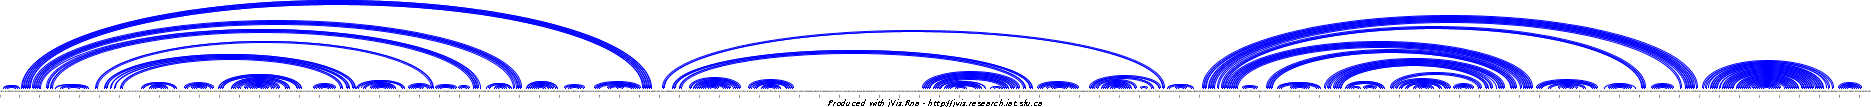
\includegraphics[width=1\textwidth, height=2cm]{../img/human-linear}
  \caption{Spojnicový graf}
  \label{obr:human_linked}
\end{figure}

\begin{figure}
  \centering
  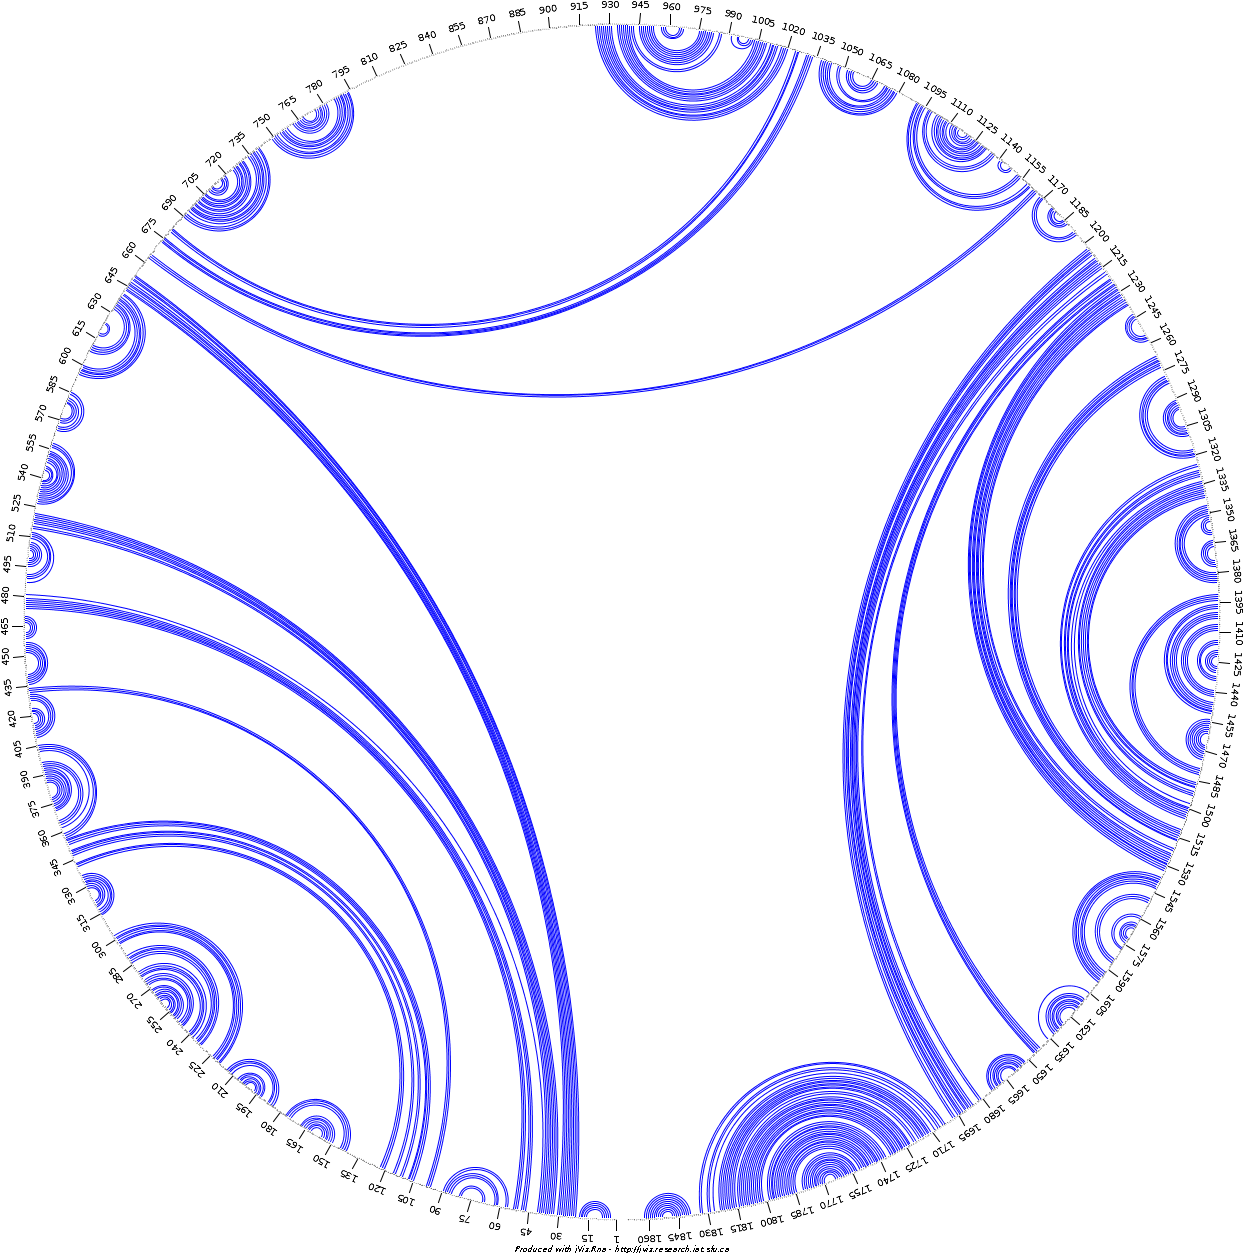
\includegraphics[width=0.7\textwidth]{../img/human-circular}
  \caption{Kruhový graf}
  \label{obr:human_circular}
\end{figure}

\begin{figure}
  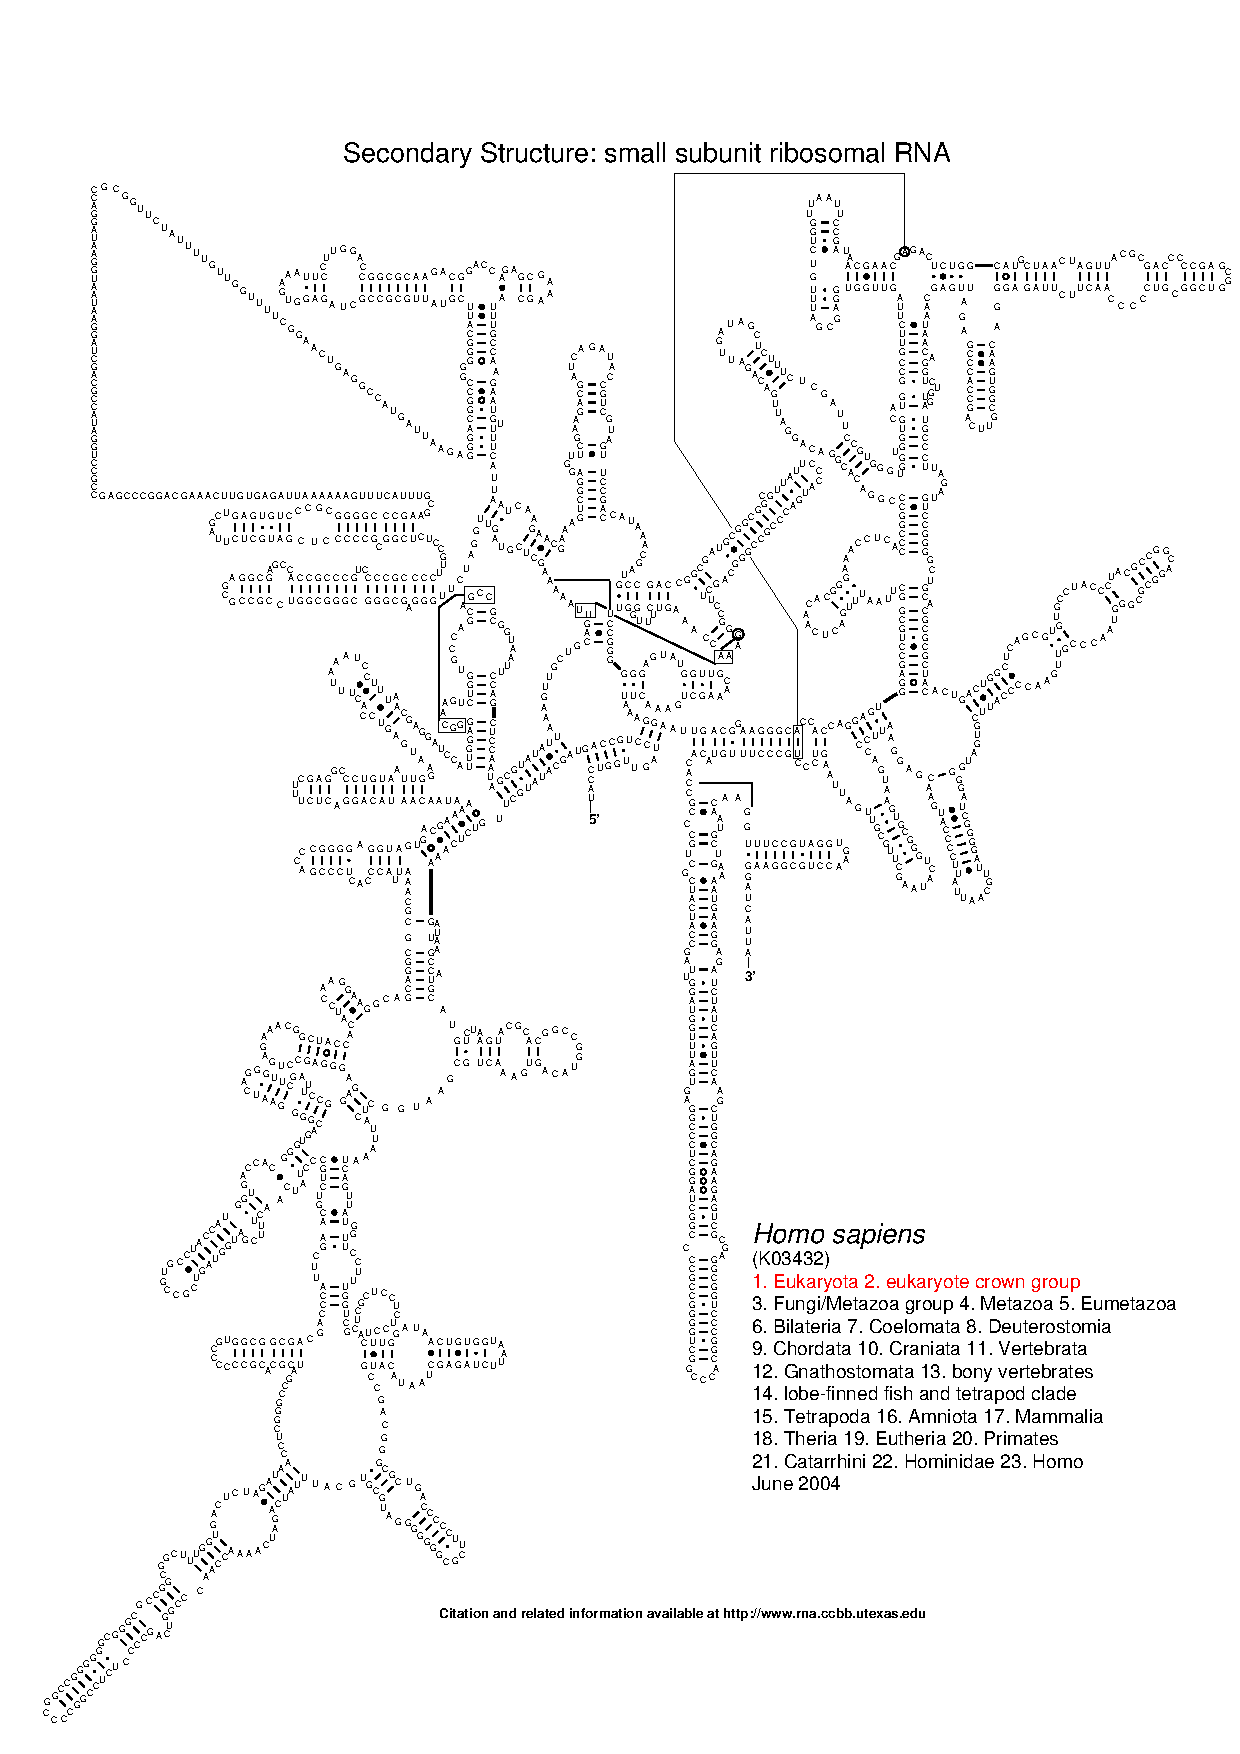
\includegraphics[width=1\textwidth]{../img/human_crw}
  \caption{Vizualizácia sekundárnej štruktúry RNA človeka z CRW databázy \citenum{CRW}}
  \label{obr:human_crw}
\end{figure}




\subsection{Motívy}

Niektoré časti molekuly vytvárajú isté motívy, z~ktorých niektoré môžeme
vidieť na obrázku \ref{obr:RNA_motifs}.
Motívom sú aj pseudouzly \ref{obr:pseudoknot_types}, ale v~tejto práci
sa nimi nebudeme zaoberať.

Stem (stonka) je časť molekuly, kde sa na seba párujú dva súvislé časti vlákna.
Loopom budeme označovať miesta s nespárovanými bázami.
Bulge (vypuklina) je miesto v~steme, ktoré z~jednej strany obsahuje loop.
Podobná je interior (vnútorná) loop, tá ale má loop po oboch stranách stemu.
Hairpin je stem zakončený loopom a~nakoniec multibranch (viac vetvová) loop
je podobná ako interior loop, ale spája dokopy viac stemov.
V~ďalšom rozprávaní nám bude stačiť rozdelenie na stem (spárované bázy)
a~loop (nespárované bázy).

\begin{figure}
  \centering
  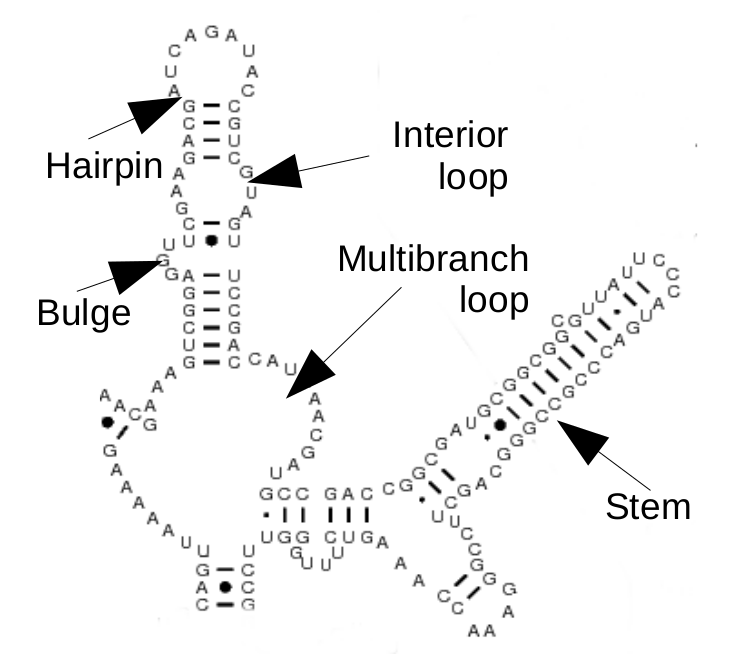
\includegraphics[width=70mm, height=70mm]{../img/struktury_v_rna.png}
  \caption{Štrukturálne motívy v RNA}
  \label{obr:RNA_motifs}
\end{figure}


\begin{figure}
%trim=left bottom right top
  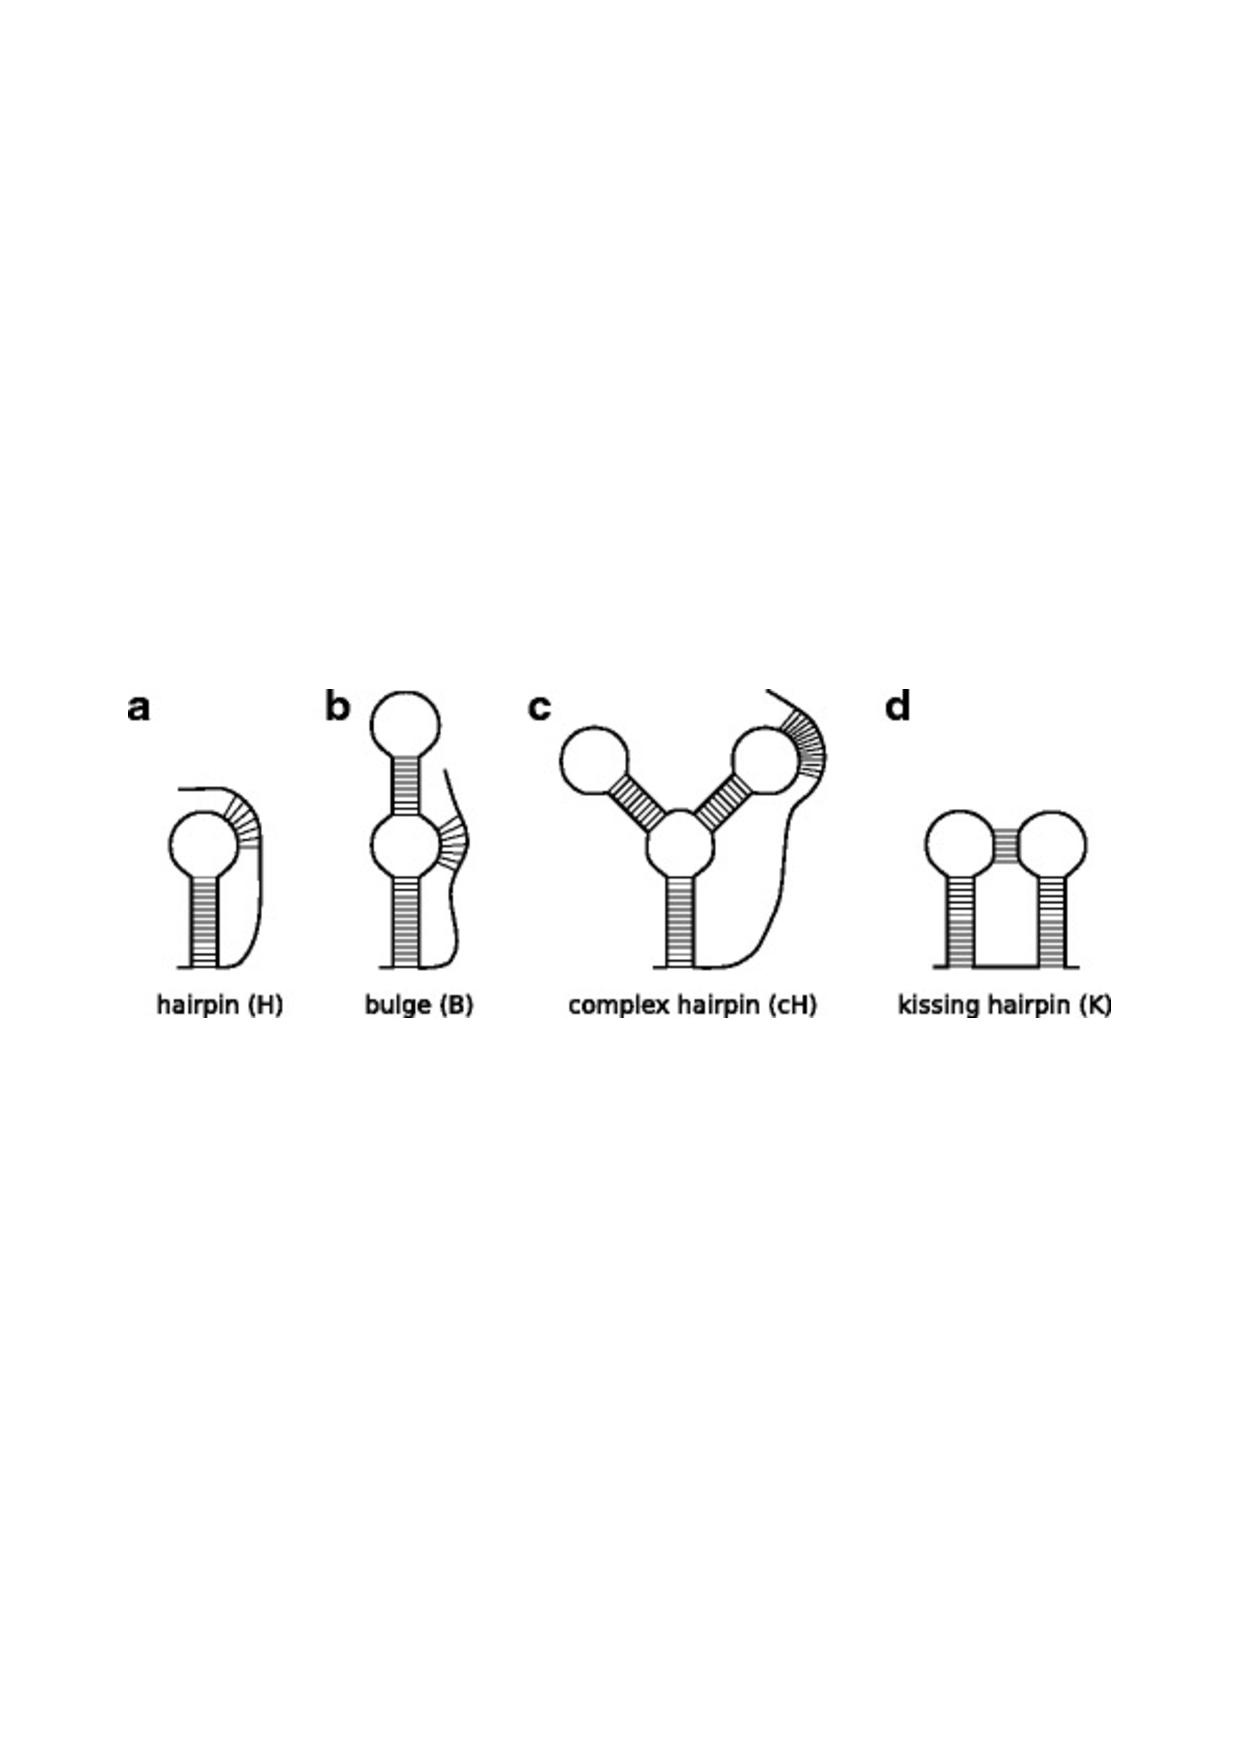
\includegraphics[clip, trim=0 12cm 0 11cm, width=0.9\textwidth]{../img/pseudoknot}
  \caption{Typy pseudouzlov podľa \citenum{PSEUDOKNOT_TYPES}}
  \label{obr:pseudoknot_types}
\end{figure}




\section{Hlavný objekt záujmu - rRNA}

Ako hlavný objekt záujmu sme si spomedzi všetkych druhov RNA vybrali práve ribozomálnu, rRNA.
Jej funkcia je hlavne v~translácií génov, pri ktorej sa genetická informácia prekladá
z~poradia nukleotidov v~mRNA do poradia aminokyselín v~bielkovine.

\begin{figure}[H]
  \centering
  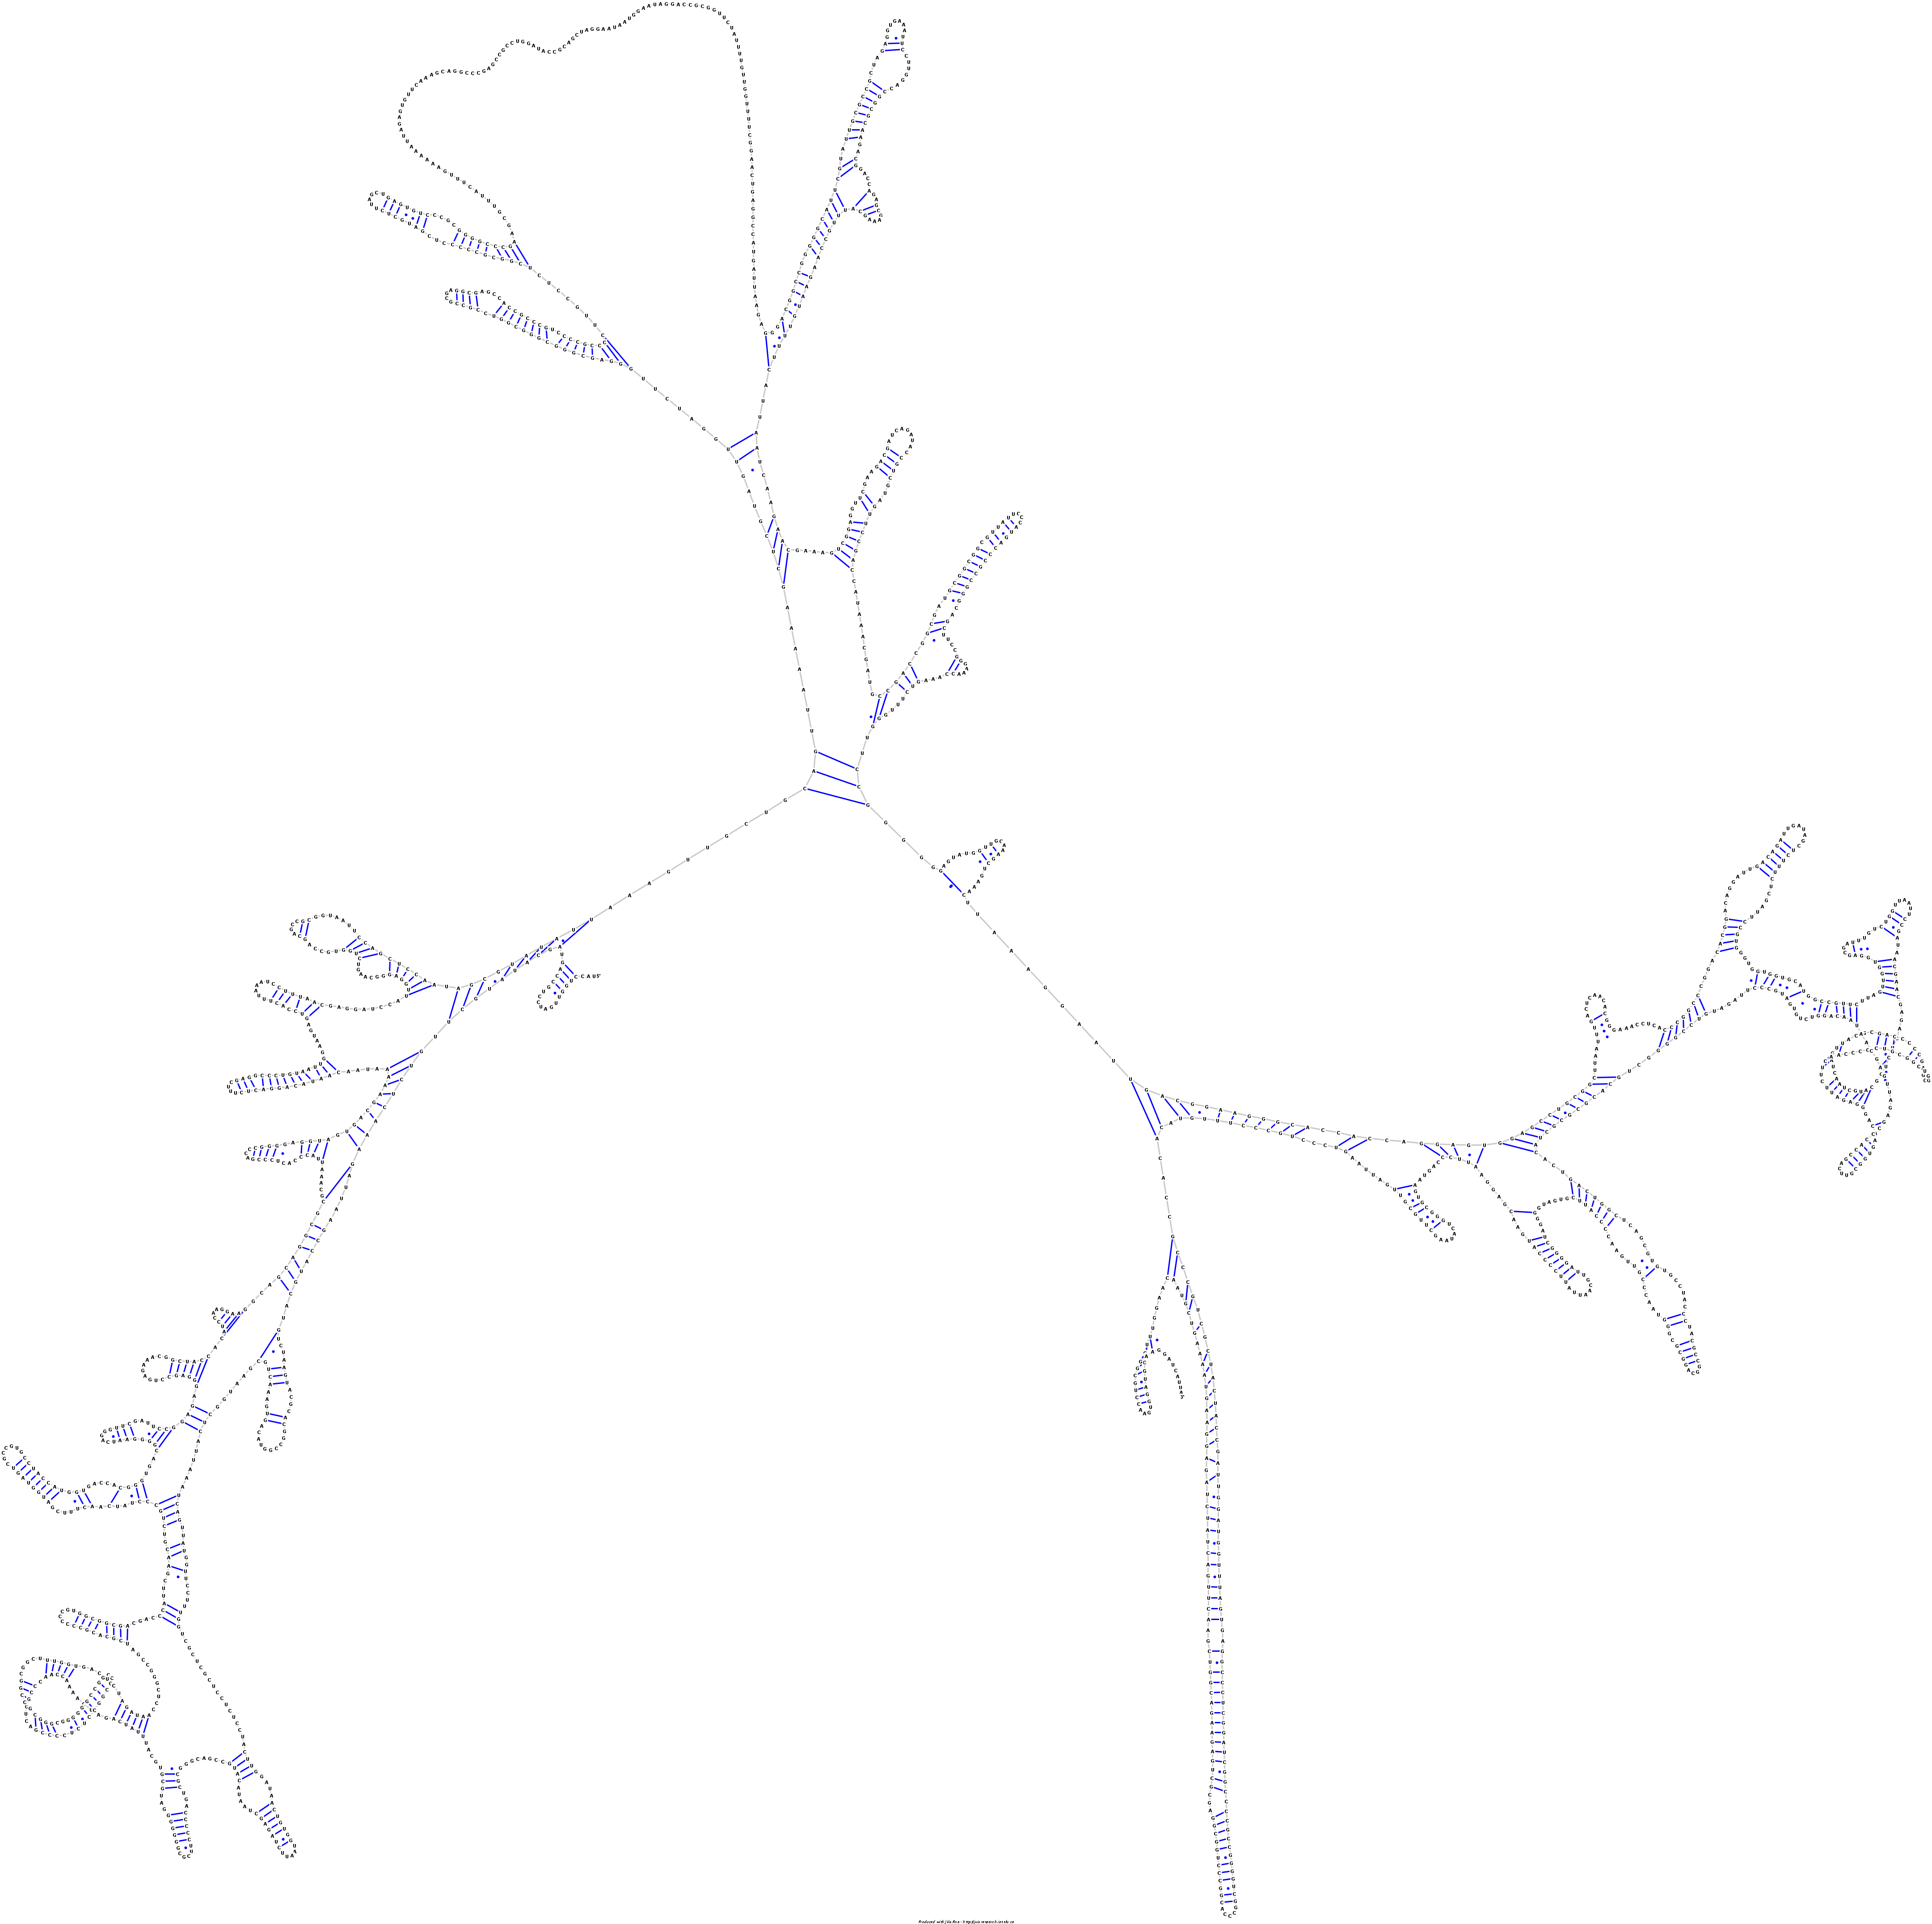
\includegraphics[width=0.9\textwidth]{../img/human_jviz}
  \caption{Malá podjednotka vygenerovaná programom jViz.Rna \citenum{JVIZ}}
  \label{obr:human_jviz}
\end{figure}

\begin{figure}
%trim=left bottom right top
  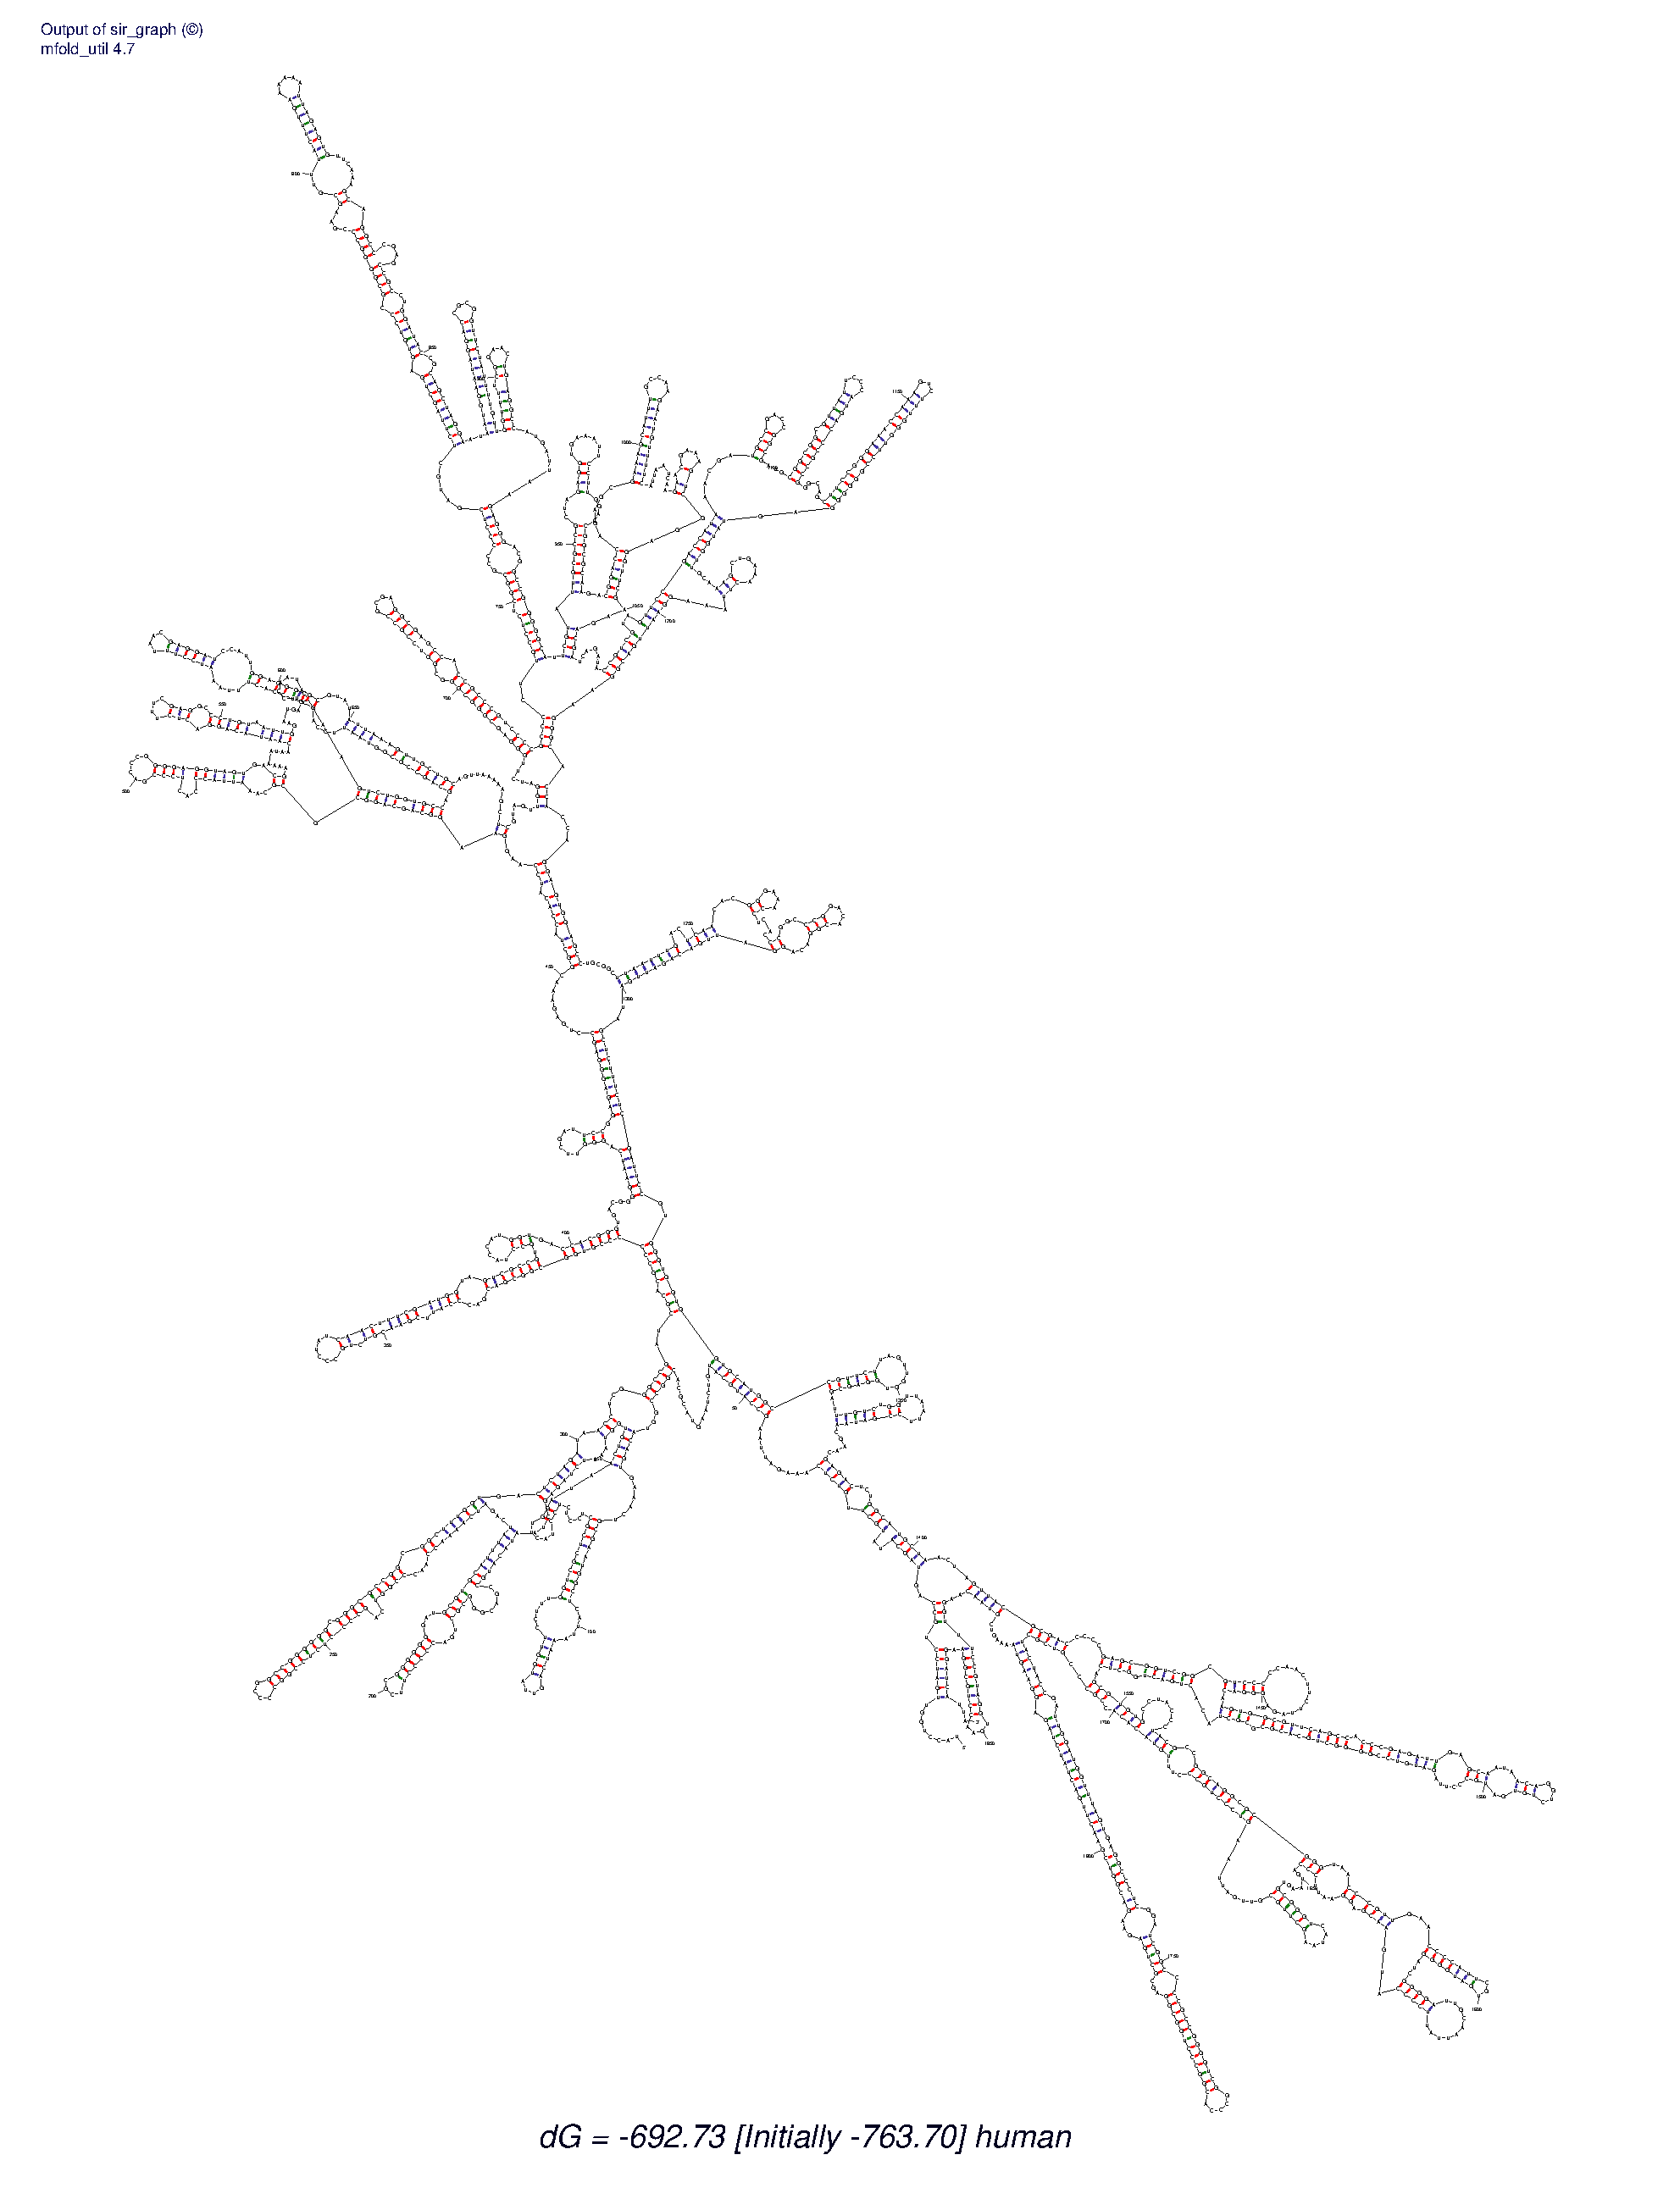
\includegraphics[trim=0 0 2cm 0, width=1\textwidth]{../img/human_mfold}
  \caption{Malá podjednotka vygenerovaná programom Mfold \citenum{MFOLD}}
  \label{obr:RNA_human_mfold}
\end{figure}

\begin{figure}
%trim=left bottom right top
  \centering
  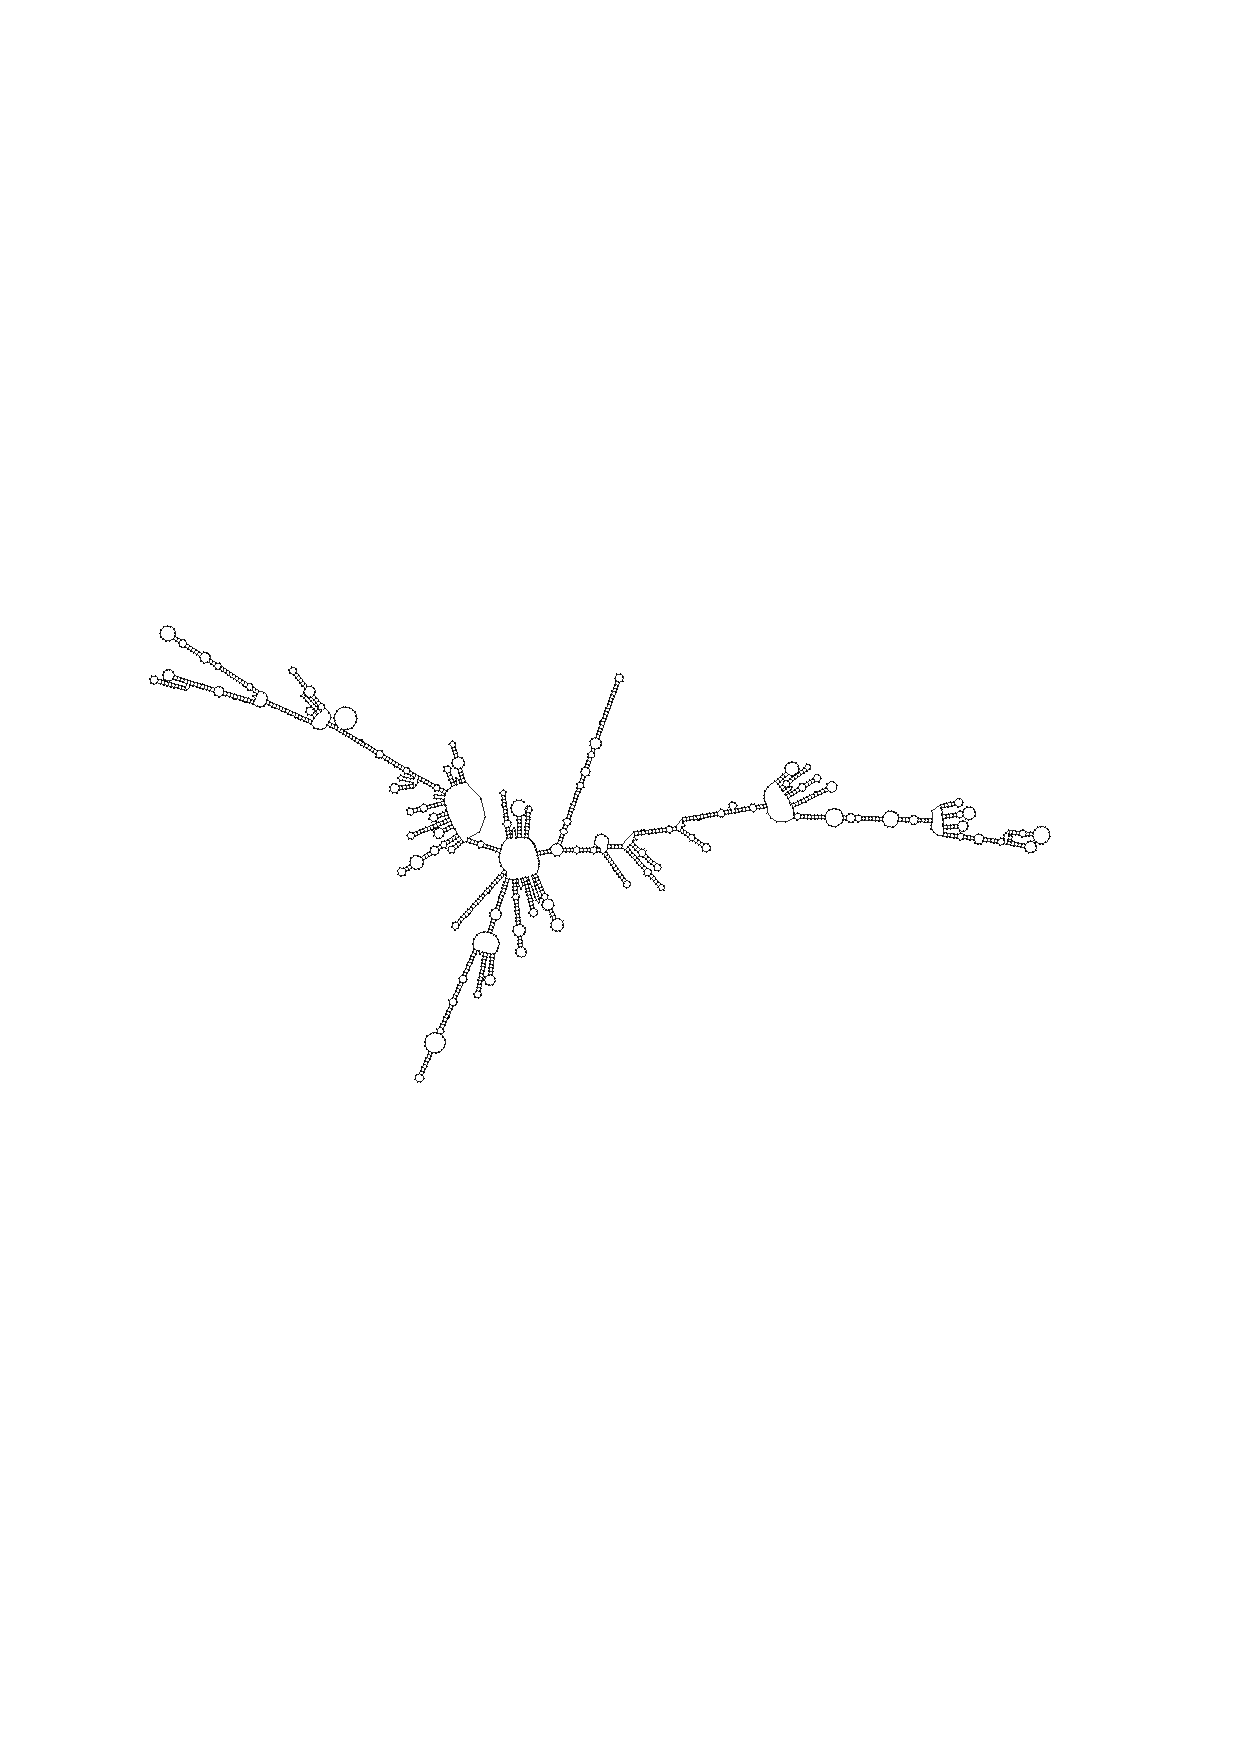
\includegraphics[clip, trim=2.5cm 10cm 3cm 10cm, angle=90, width=1\textwidth]{../img/human_RNAfold}
  \caption{Malá podjednotka vygenerovaná programom RNAfold \citenum{VIENNA_RNA}}
  \label{obr:RNA_human_rnafold}
\end{figure}

Zvolili sme si ju taktiež kvôli jej konzervovanosti naprieč evolučným spektrom. Ďalším
dôvodom bola jej veľkosť, ktorá robí existujúcim nástrojom najväčšie problémy
pri vizualizácií. Na obrázku \ref{obr:human_crw} vidíme sekundárnu štruktúru 
K03432 malej podjednotky ribozomálnej RNA človeka z~CRW databázy.
Tá znázorňuje predstavy biológov o~tom, ako by malo nakreslenie danej molekuly vyzerať.
Obrázky \ref{obr:human_jviz}, \ref{obr:RNA_human_mfold} a~\ref{obr:RNA_human_rnafold}
sú zase vygenerované vizualizácie pomocou programov jViz.Rna, Mfold a~RNAfold.
Dodržiavanie základných kritérií ako rovinnosť, loopy na kružniciach a~stemy na priamkach
sa prevažne programom darí, no celkový vzhľad obrázkov je úplne odlišný od požiadavok
biológov, keďže sa motívy z~obrázka z~CRW databázy hľadajú veľmi ťažko.





\section{Stromová reprezentácia sekundárnej štruktúry}

Vďaka ignorovaniu pseudouzlov v~definícií \ref{def:RNA_sekundarna_struktura} sekundárnej
štruktúry ju môžeme reprezentovať ako usporiadaný strom
\footnote{Používame pojmy z~nasledujúcej kapitoly \nameref{kap:grafy}}.

Bez straty všeobecnosti budeme vždy hovoriť ako o~strome, aj keď sa môže stať
(a~typicky aj stáva), že štruktúra nebude celistvá, teda nejde o~strom, ale o~les.
V~tom prápade môžeme pripojiť nový špeciálny koreňový vrchol, ktorého potomkovia
(viz. definícia \ref{def:stromove_pojmy}) budú dané stromy a~ktorý nebudeme vizualizovať.

Na obrázku \ref{obr:RNA_stromova_reprezentacia} vidíme varianty reprezentácie vrcholov.
Tie môžu zastupovať celé motívy, alebo iba nukleotid, respektíve celý bázový pár.

\begin{figure}
  \centering
  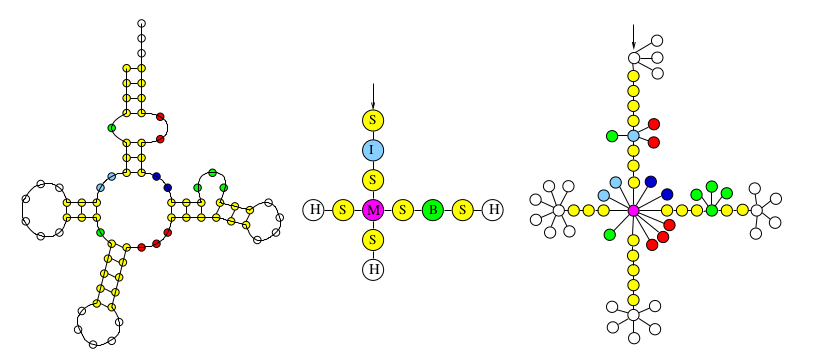
\includegraphics[width=130mm, height=70mm]{../img/stromova_reprezentacia_rna}
  \caption{Varianty reprezentácie vrcholov podľa \citenum{RNA_DRAW}}
  \label{obr:RNA_stromova_reprezentacia}
\end{figure}

V~našej práci vrchol stromu reprezentuje bázový pár (vnútorný vrchol)
alebo nespárovanú bázu (list stromu), ako je to zobrazené na obrázku \ref{obr:rna_to_tree}
Štruktúru do ktorej patrí si totiž vieme ľahko zistiť z~potomkov vrcholu.


%rna, from 5' to 3':
% AUGCAAACUGGCACCCUCAU
% (((((...))(...))..))

\begin{center}
  \begin{minipage}{.500\textwidth}
    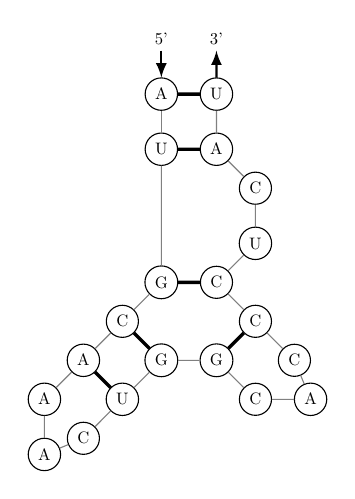
\begin{tikzpicture}[
        on grid,
        node distance = 0.7,
        -latex,
        scale = \scale,
        every node/.style = {scale = \scale},
        base/.style = {circle, draw},
        ends/.style = {draw = none, fill = none}]

      %ends, 5' a 3'
      \node[ends] (5end) {5'};
      \node[ends] (3end) [right = of 5end] {3'};

      %stem
      \node[base] (StemLeft1) [below = of 5end] {A};
      \node[base] (StemRight1) [right = of StemLeft1] {U};
      \node[base] (StemLeft2) [below = of StemLeft1] {U};
      \node[base] (StemRight2) [right = of StemLeft2] {A};

      %bulge
      \node[base] (Bulge1) [below right = of StemRight2] {C};
      \node[base] (Bulge2) [below = of Bulge1] {U};

      %stem
      \node[base] (StemRight3) [below left = of Bulge2] {C};
      \node[base] (StemLeft3) [left = of StemRight3] {G};

      %left-branch
      \node[base] (LBranchLStem1) [below left = of StemLeft3] {C};
      \node[base] (LBranchRStem1) [below right = of LBranchLStem1] {G};
      \node[base] (LBranchLStem2) [below left = of LBranchLStem1] {A};
      \node[base] (LBranchRStem2) [below left = of LBranchRStem1] {U};

      %left-branch-hairpin
      \node[base] (LBranchHairpin1) [below left = of LBranchLStem2] {A};
      \node[base] (LBranchHairpin2) [below = of LBranchHairpin1] {A};
      \node[base] (LBranchHairpin3) [below left = of LBranchRStem2] {C};

      %right-branch
      \node[base] (RBranchRStem1) [below right = of StemRight3] {C};
      \node[base] (RBranchLStem1) [below left = of RBranchRStem1] {G};

      %right-branch-hairpin
      \node[base] (RBranchHairpin1) [below right = of RBranchLStem1] {C};
      \node[base] (RBranchHairpin2) [right = of RBranchHairpin1] {A};
      \node[base] (RBranchHairpin3) [below right = of RBranchRStem1] {C};

      \begin{scope}[-]
      %pair edges
        \path[very thick]
        (StemLeft1) edge (StemRight1)
        (StemLeft2) edge (StemRight2)
        (StemLeft3) edge (StemRight3)
        (LBranchLStem1) edge (LBranchRStem1)
        (LBranchLStem2) edge (LBranchRStem2)
        (RBranchLStem1) edge (RBranchRStem1)
        ;
      %lines around molecule
        \path[color = gray]
        (StemLeft1) edge (StemLeft2)
        (StemLeft2) edge (StemLeft3)
        (StemLeft3) edge (LBranchLStem1)
        (LBranchLStem1) edge (LBranchLStem2)
        (LBranchLStem2) edge (LBranchHairpin1)
        (LBranchHairpin1) edge (LBranchHairpin2)
        (LBranchHairpin2) edge (LBranchHairpin3)
        (LBranchHairpin3) edge (LBranchRStem2)
        (LBranchRStem2) edge (LBranchRStem1)
        (LBranchRStem1) edge (RBranchLStem1)
        (RBranchLStem1) edge (RBranchHairpin1)
        (RBranchHairpin1) edge (RBranchHairpin2)
        (RBranchHairpin2) edge (RBranchHairpin3)
        (RBranchHairpin3) edge (RBranchRStem1)
        (RBranchRStem1) edge (StemRight3)
        (StemRight3) edge (Bulge2)
        (Bulge2) edge (Bulge1)
        (Bulge1) edge (StemRight2)
        (StemRight2) edge (StemRight1)
        ;
      \end{scope}

      \begin{scope}
        % edges to ends
        \path[thick]
        (5end) edge (StemLeft1)
        (StemRight1) edge (3end)
        ;
      \end{scope}
    \end{tikzpicture}
  \end{minipage}
  \begin{minipage}{.450\textwidth}
    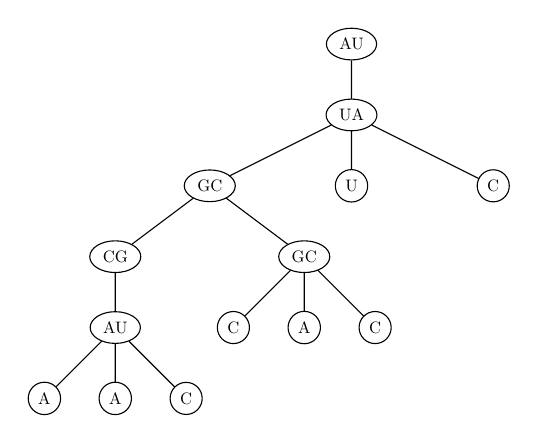
\begin{tikzpicture}[
        baseline,
        level distance = 1.5 cm,
        scale = \scale,
        every node/.style = {scale = \scale},
        basepair/.style = {ellipse, draw, minimum height = 0.3 cm, minimum width = 0.7 cm},
        unpaired/.style = {circle, draw, minimum width = 0.3 cm},
        level 2/.style = {sibling distance = 3 cm},
        level 3/.style = {sibling distance = 4 cm},
        level 4/.style = {sibling distance = 1.5 cm}
      ]
      \node[basepair] {AU}
      child {
        node[basepair] {UA}
        child {
          node[basepair] {GC}
          child {
            node[basepair] {CG}
            child {
              node[basepair] {AU}
              child {
                node[unpaired] {A}
              }
              child {
                node[unpaired] {A}
              }
              child {
                node[unpaired] {C}
              }
            }
          }
          child {
            node[basepair] {GC}
            child {
              node[unpaired] {C}
            }
            child {
              node[unpaired] {A}
            }
            child {
              node[unpaired] {C}
            }
          }
        }
        child {
          node[unpaired] {U}
        }
        child {
          node[unpaired] {C}
        }
      }
      ;
    \end{tikzpicture}
      %\caption{Stromova reprezentacia RNA}
      %\label{obr:RNA_tree}
  \end{minipage}
\end{center}






\section{Grafové pojmy}
\label{kap:grafy}

V~tejto časti zadefinujeme pojmy a~značenie, ktoré budeme v~tejto práci používať.
Z~väčšej časti ho prevezmeme od \citet{RTED}.

\begin{definice}\label{def:strom}
  Usporiadaný zakorenený strom je orientovaný graf bez cyklov,
  jeho hrany sú orientované vždy v smere od koreňa, t.j. z~predka k~potomkovi.

  Okrem koreňa má každý vrchol svojho predka a~existuje usporiadanie medzi potomkami.

  Usporiadany les je usporiadaná množina stromov.
\end{definice}

Ak \tree{F} je les, $V_F$ budeme označovať množinu jeho vrcholov a $E_F$ množinu jeho hrán.
Prázdny strom/les budeme značiť $\emptyset$.

\begin{definice}
  \label{def:stromove_pojmy}
  Nech \tree{F} je strom, $u$ a $v$ jeho dva rôzne vrcholy.
  Hovoríme, že $u$ je predkom (rodičom) $v$ ($v$ je potomok $u$) ak $(u, v) \in E_{\tree{F}}$.
  Hovoríme, že $u$ je súrodencom $v$, ak sú to rôzne vrcholy a majú spoločného predka.
\end{definice}

Vnútornými vrcholmi budeme označovať vrcholy, ktoré majú nejakého potomka,
tie bez potomkov nazveme listy.

Podles lesa \tree{F} je les \tree{G} s~vrcholmi $V_{\tree{G}} \subseteq V_{\tree{F}}$
a~hranami $E_{\tree{G}} \subseteq E_{\tree{F}} \cap (V_{\tree{G}} \times V_{\tree{G}})$.
Obdobne to plati aj pre podstrom stromu.

Nech $v$ je vrchol stromu \tree{F}. Potom \tree{F_{v}} budeme značiť podstrom \tree{F} zakorenený vo $v$,
t.j. v~strome ostávajú potomkovia $v$, ich potomkovia, atď.
\tree{F - v} budeme značiť les, ktorý vznikne zmazaním vrcholu $v$ z \tree{F} spolu so
všetkými hranami obsahujúcimi $v$. Podobne \tree{F - \tree{F_{v}}} budeme značiť les, ktorý
dostaneme zmazaním podstromu \tree{F_{v}} z~\tree{F}.

\begin{definice}[Root-leaf cesta]
  Nech je $F$ strom. Cestou v~$F$ nazveme jeho súvislý podgraf taký, že všetky jeho vrcholy
  majú stupeň najviac 2.

  Root-leaf cestou v $F$ budeme nazývať cestu začínajúcu v koreni stromu \sloppy\mbox{a končiacu}
  v~nejakom jeho liste.
\end{definice}

V práci budeme využívať tri druhy ciest, budú to $left, right, heavy$ a~označovať ich
budeme $\gamma^L, \gamma^R, \gamma^H$. $Left$ bude v~strome cesta idúca vždy do prvého (ľavého)
potomka, $right$ do posledného (pravého) a~$heavy$ zase cesta idúca do vrcholu s~najväčším
podstromom (najťažším)\footnote{ťažkých ciest môže existovať aj viac ako jedna}.

Príklad $root$-$leaf$ cesty v~strome je na obrázku \ref{obr:root_leaf_path}.



\begin{figure}[H]
  \centering
  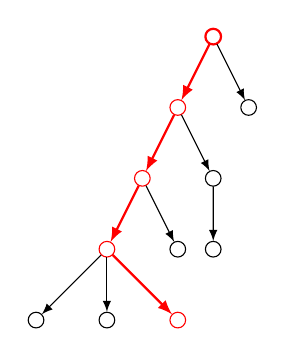
\begin{tikzpicture}[
      on grid,
      -latex,
      font=\large,
      scale = \scale,
      level distance = 1.5 cm,
      every node/.style = {scale = \scale, circle, draw, thin},
      colored/.style = {color = red, thick},
      black/.style = {color = black, thin}]

      \node [colored]{}
      child[colored] {
        node {}
        child[colored] {
          node{}
          child {
            node{}
            child[black] {
              node{}
            }
            child[black] {
              node{}
            }
            child {
              node{}
            }
          }
          child[black] {
            node{}
          }
        }
        child[black] {
          node{}
          child {
            node{}
          }
        }
      }
      child[black] {
        node{}
      }
      ;
  \end{tikzpicture}
  \caption{Príklad stromu. Je v ňom červene vyznačená $heavy$ cesta}
  \label{obr:root_leaf_path}
\end{figure}



